\documentclass[../../main.tex]{subfiles}

\graphicspath{{../../fig/}}
\setcounter{section}{0}

\begin{document}
\chapter{スパースワイヤーグリッドのたわみ量の評価}
\label{chap:wiresag_swg}
\ref{}章にて、ワイヤーのたわみ量を自動で評価する装置を開発した。
本章では、開発した装置を用いて実際に偏光角較正に使用されるスパースワイヤーグリッドのたわみ量を評価する。
はじめに、評価するスパースワイヤーグリッドの作成方法について述べ、次いで評価結果とその考察を行う。
その後、評価されたたわみ量が大きかったものについて修繕を加え、再度評価を行った結果について述べる。
最後に、今回のたわみ量の評価を通じて得られた、スパースワイヤーグリッドの作成方法に関する今後の展望について述べる。

\section{評価されたスパースワイヤーグリッドの詳細}
今回評価したスパースワイヤーグリッドは、\ref{subsec:wg_design}項で述べたように$\SI{230}{g}$の重りを使用し、
ワイヤー番号が奇数番目のものと偶数番目のものに分け、二回に分けてワイヤーを張ることで作成された。
このとき、はじめにワイヤー番号が奇数番目のものを張り、次にワイヤー番号が偶数番目のものを張った。
作成されたスパースワイヤーグリッドを装置に取り付けた様子を図\ref{fig:wiresag_swg_sparse_wiregrid}に示す。
なお、\ref{chap:wiresag}章にて述べたように一度に測定できるのはスパースワイヤーグリッドの半面のみであるので、
ワイヤー番号が$0\sim19$番のワイヤーと$20\sim38$番のワイヤーに分けて測定を行った。
\begin{figure}[tbp]
    \centering
    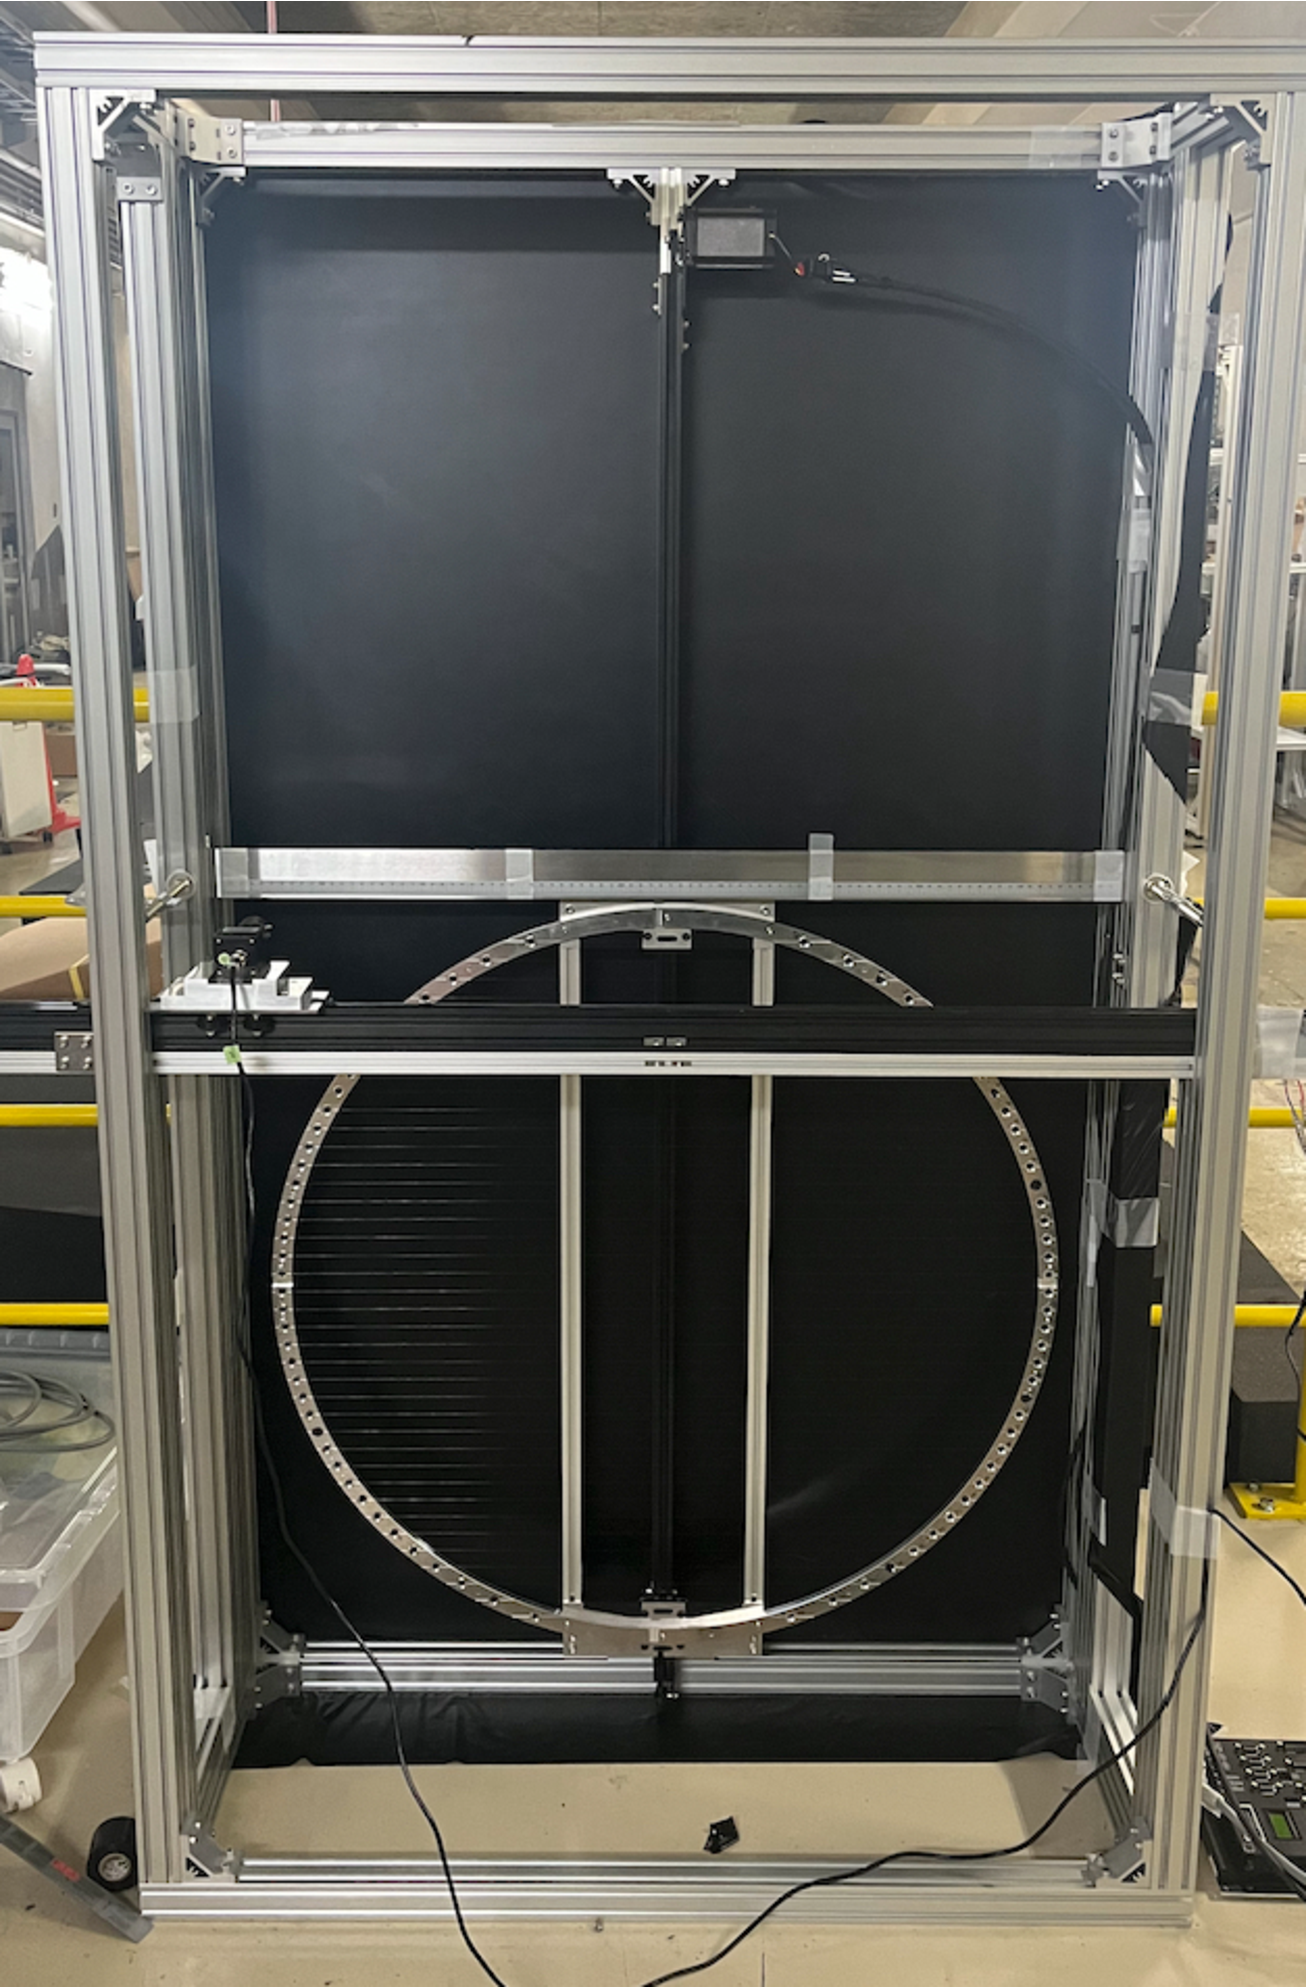
\includegraphics[width=0.6\textwidth]{wiresag_swg/wiresag_sparse_wiregrid.pdf}
    \caption{スパースワイヤーグリッドのたわみ量の評価の様子}
    \label{fig:wiresag_swg_sparse_wiregrid}
\end{figure}
\subsection{評価結果とその考察}
図\ref{fig:wiresag_swg_result}(\subref{fig:wiresag_swg_sag_result})にスパースワイヤーグリッドのたわみ量の評価結果を示す。
横軸はワイヤー番号、縦軸はワイヤーのたわみ量を示している。
fitting errorを統計的な誤差として、前章にて得られた$\SI{50}{\mu m}$を系統的な誤差として、それらの2乗和をたわみ量の誤差として。
図中には測定されたたわみ量に加え、理論値として$\SI{230}{g}$の重りによって生まれるたわみ量を、
たわみ角が$0.3\tcdegree,\,0.5\tcdegree$になるたわみ量を示している。
また、図\ref{fig:wiresag_swg_result}(\subref{fig:wiresag_swg_sag_angle_result})に
評価されたたわみ量をたわみ角に変換した結果を示す。
横軸はワイヤー番号、縦軸はワイヤーのたわみ角を示している。
図中には測定されたたわみ角に加え、たわみ角が$0.3\tcdegree,\,0.5\tcdegree$の線を示している。
測定されたたわみ角の平均は$0.25\tcdegree$であり、たわみ角の誤差の平均は$0.05\tcdegree$であった。
ほとんどのワイヤーについて、そのたわみ角が$0.3\tcdegree$以下であることがわかる。
\begin{figure}[H]
    \begin{minipage}[b]{0.5\hsize}
        \centering
        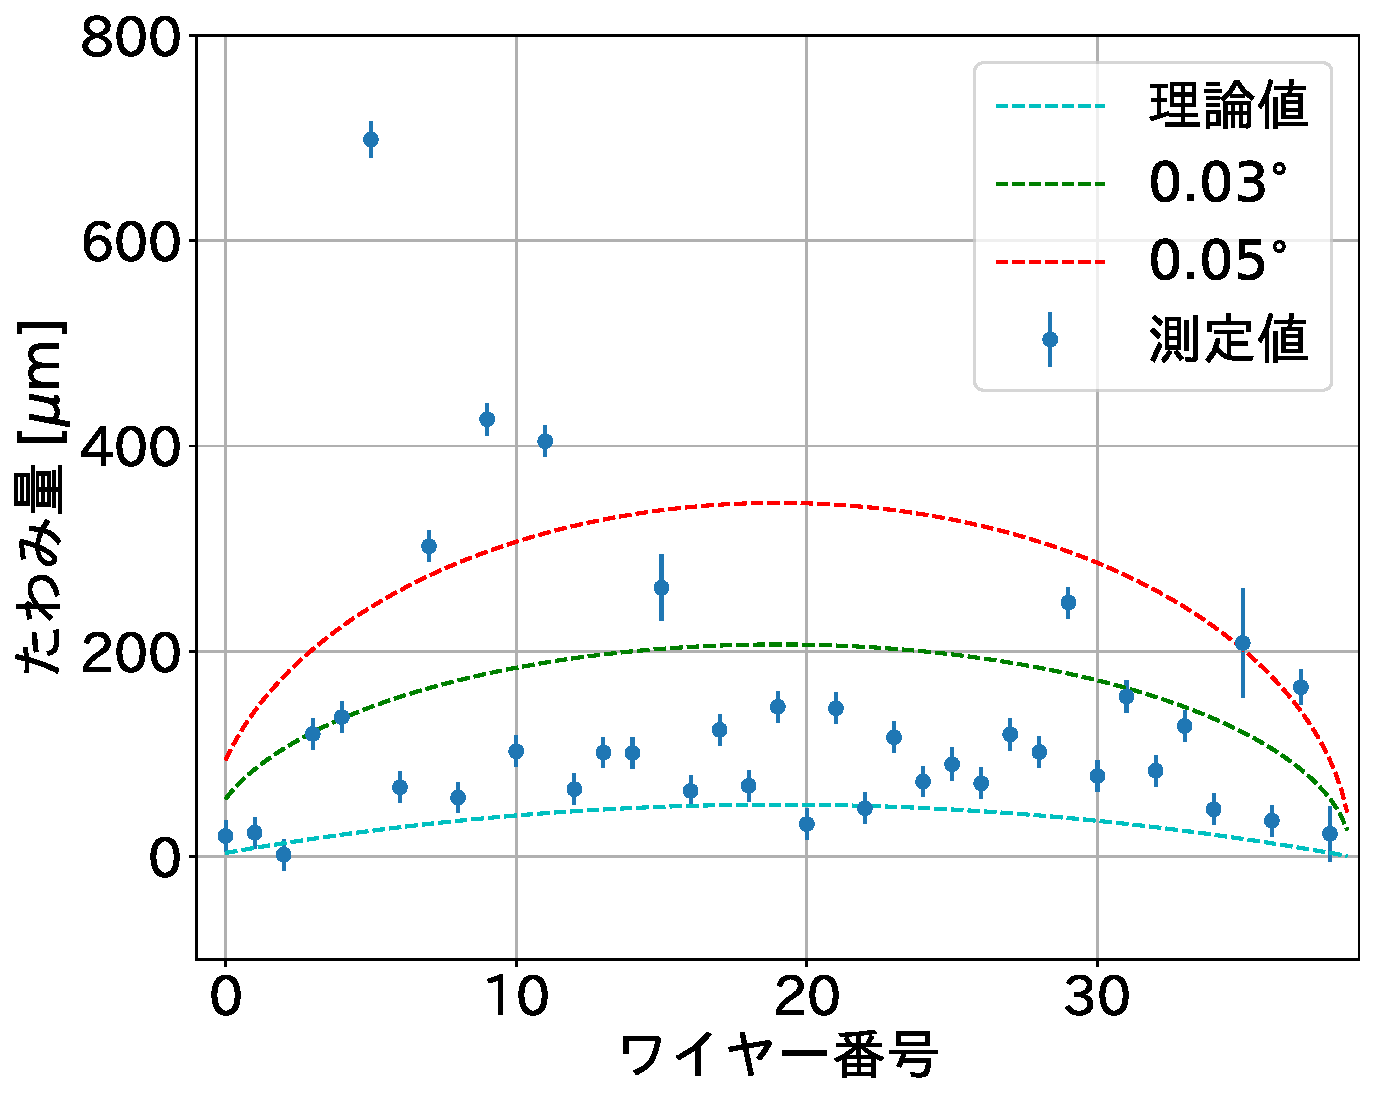
\includegraphics[width=1.0\textwidth]{wiresag_swg/swg_sag_before.pdf}
        \subcaption{}
        \label{fig:wiresag_swg_sag_result}
    \end{minipage}
    \begin{minipage}[b]{0.5\hsize}
        \centering
        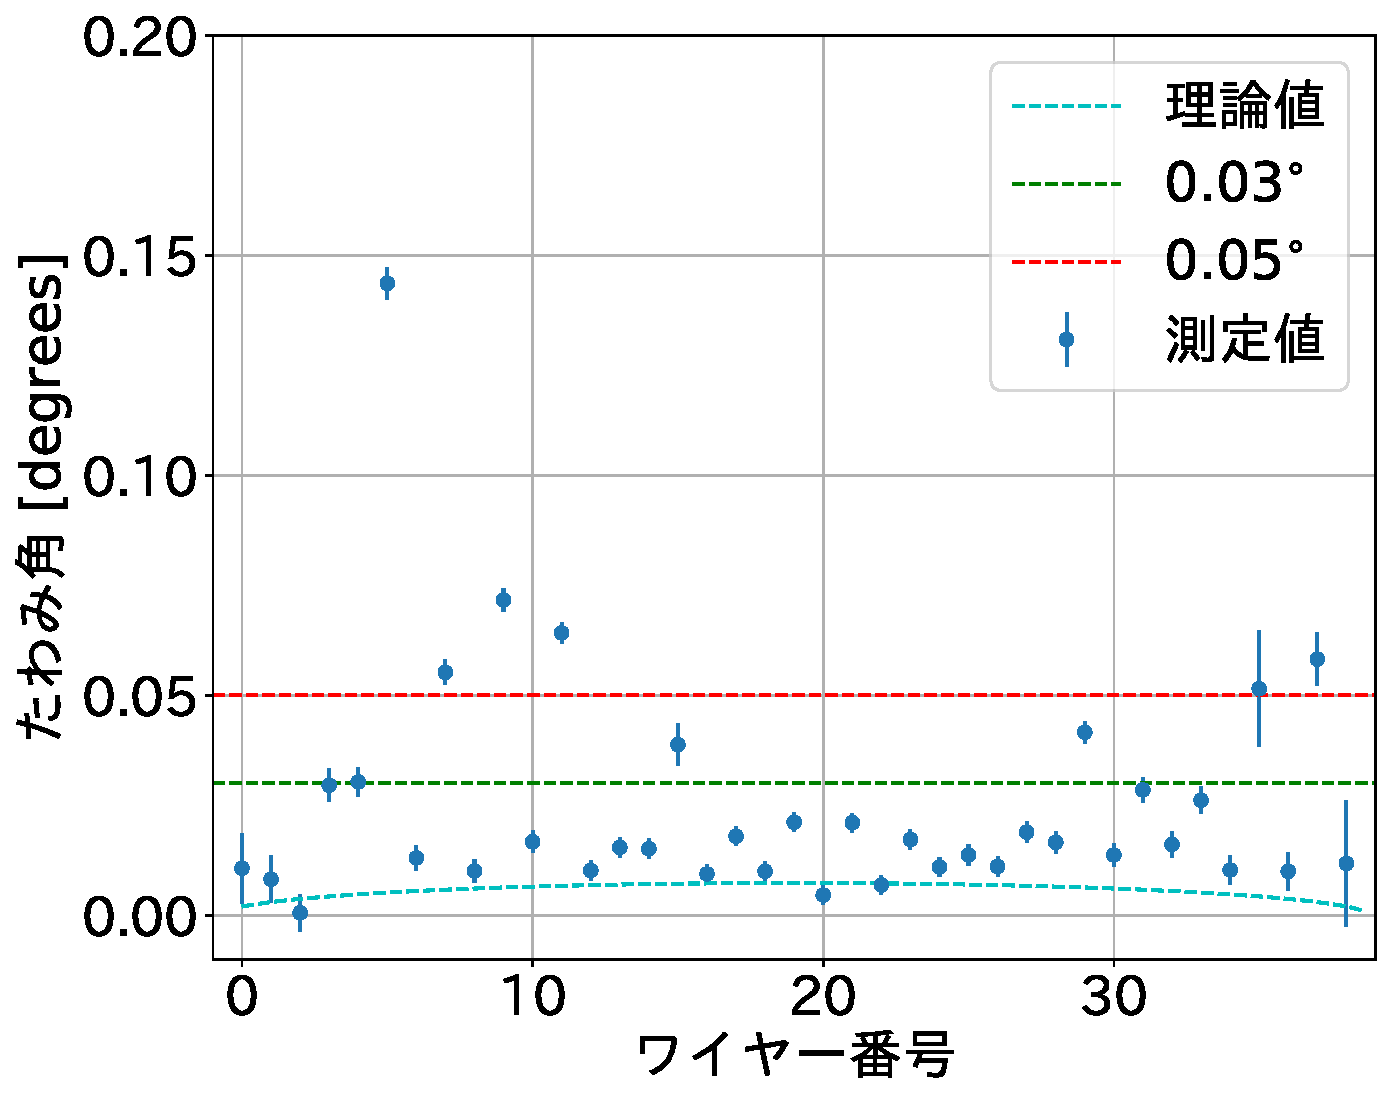
\includegraphics[width=1.0\textwidth]{wiresag_swg/swg_sag_angle_before.pdf}
        \subcaption{}
        \label{fig:wiresag_swg_sag_angle_result}
    \end{minipage}
    \caption{(\subref{fig:wiresag_swg_sag_result}) スパースワイヤーグリッドのたわみ量の評価結果\ 
             (\subref{fig:wiresag_swg_sag_angle_result}) スパースワイヤーグリッドのたわみ角の評価結果}
    \label{fig:wiresag_swg_result}
\end{figure}




\end{document}